\documentclass{standalone}
\usepackage{tikz}
\usetikzlibrary{patterns, positioning}


\begin{document}
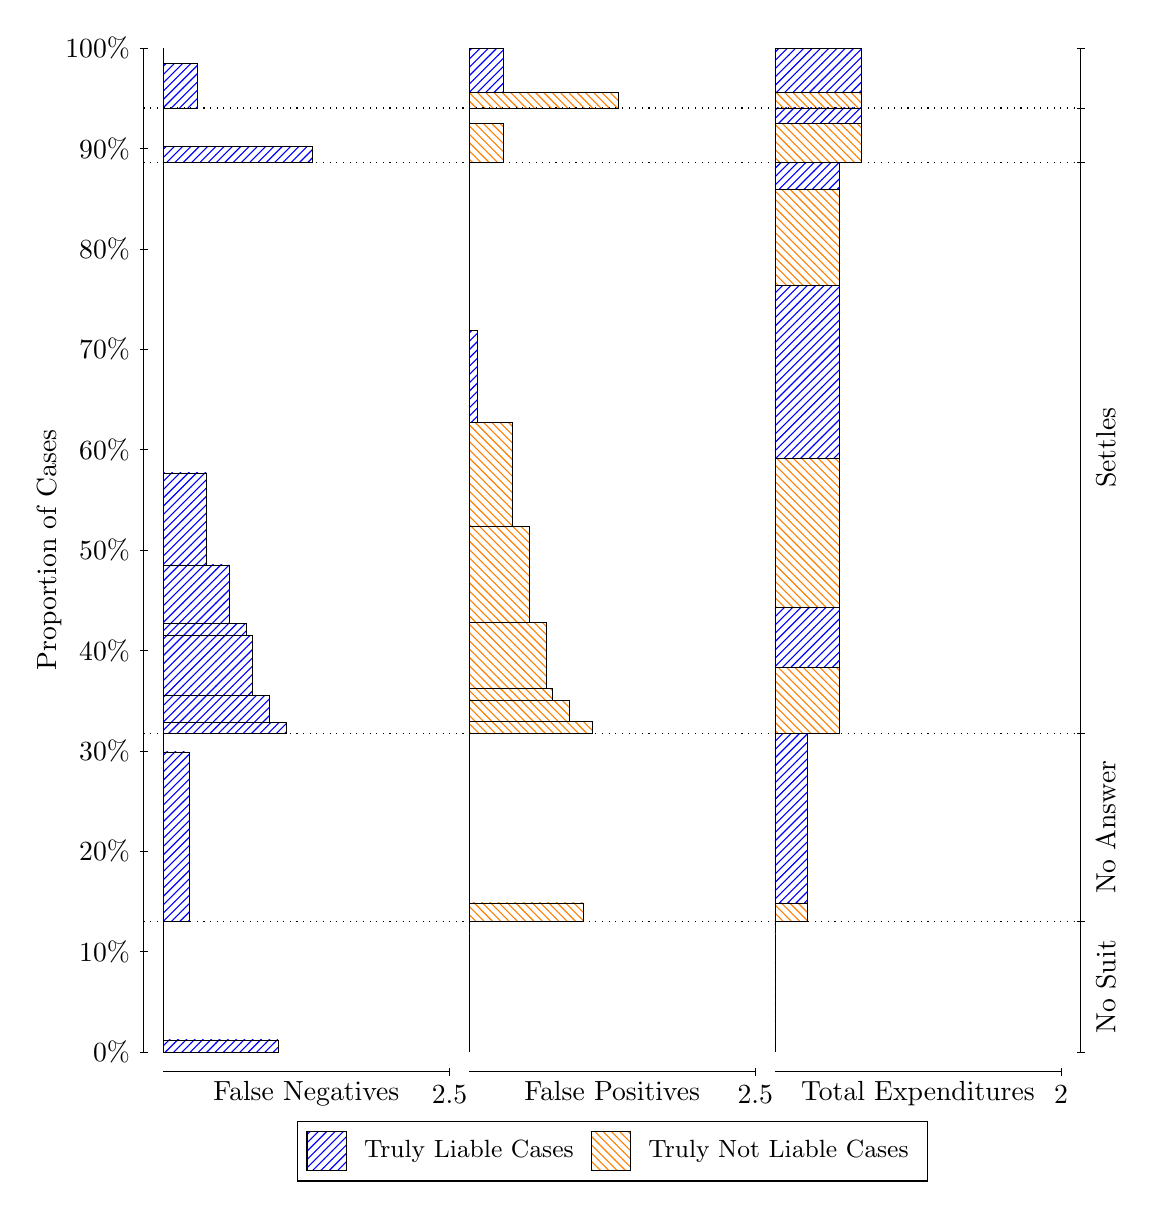
\begin{tikzpicture}
\draw[black, very thin] (1.5,1.75) -- (1.5,14.5);
\node[rotate=90, text=black, anchor=center] at (0.3, 8.125) {Proportion of Cases};
\draw[black, very thin] (1.45,1.75) -- (1.55,1.75);
\node[text=black, anchor=east] at (1.45, 1.75) {0\%};
\draw[black, very thin] (1.45,3.025) -- (1.55,3.025);
\node[text=black, anchor=east] at (1.45, 3.025) {10\%};
\draw[black, very thin] (1.45,4.3) -- (1.55,4.3);
\node[text=black, anchor=east] at (1.45, 4.3) {20\%};
\draw[black, very thin] (1.45,5.575) -- (1.55,5.575);
\node[text=black, anchor=east] at (1.45, 5.575) {30\%};
\draw[black, very thin] (1.45,6.85) -- (1.55,6.85);
\node[text=black, anchor=east] at (1.45, 6.85) {40\%};
\draw[black, very thin] (1.45,8.125) -- (1.55,8.125);
\node[text=black, anchor=east] at (1.45, 8.125) {50\%};
\draw[black, very thin] (1.45,9.4) -- (1.55,9.4);
\node[text=black, anchor=east] at (1.45, 9.4) {60\%};
\draw[black, very thin] (1.45,10.675) -- (1.55,10.675);
\node[text=black, anchor=east] at (1.45, 10.675) {70\%};
\draw[black, very thin] (1.45,11.95) -- (1.55,11.95);
\node[text=black, anchor=east] at (1.45, 11.95) {80\%};
\draw[black, very thin] (1.45,13.225) -- (1.55,13.225);
\node[text=black, anchor=east] at (1.45, 13.225) {90\%};
\draw[black, very thin] (1.45,14.5) -- (1.55,14.5);
\node[text=black, anchor=east] at (1.45, 14.5) {100\%};

\draw[black, very thin] (13.4,1.75) -- (13.4,14.5);
\draw[black, very thin] (13.35,1.75) -- (13.45,1.75);
\node[anchor=west] at (13.35, 1.75) {};
\draw[black, very thin] (13.35,3.4075) -- (13.45,3.4075);
\node[anchor=west] at (13.35, 3.4075) {};
\draw[black, very thin] (13.35,5.798) -- (13.45,5.798);
\node[anchor=west] at (13.35, 5.798) {};
\draw[black, very thin] (13.35,13.051) -- (13.45,13.051);
\node[anchor=west] at (13.35, 13.051) {};
\draw[black, very thin] (13.35,13.739) -- (13.45,13.739);
\node[anchor=west] at (13.35, 13.739) {};
\draw[black, very thin] (13.35,14.5) -- (13.45,14.5);
\node[anchor=west] at (13.35, 14.5) {};

\draw[black, very thin, pattern color=blue, pattern=north east lines] (1.75,1.75) rectangle (3.2033,1.9042);
\draw[black, very thin, pattern color=orange, pattern=north west lines] (1.75,1.9042) rectangle (1.75,3.4075);
\draw[black, very thin, pattern color=blue, pattern=north east lines] (1.75,3.4075) rectangle (2.077,5.5622);
\draw[black, very thin, pattern color=orange, pattern=north west lines] (1.75,5.5622) rectangle (1.75,5.798);
\draw[black, very thin, pattern color=blue, pattern=north east lines] (1.75,5.798) rectangle (3.3123,5.9378);
\draw[black, very thin, pattern color=blue, pattern=north east lines] (1.75,5.9378) rectangle (3.0943,6.2834);
\draw[black, very thin, pattern color=blue, pattern=north east lines] (1.75,6.2834) rectangle (2.8763,7.0448);
\draw[black, very thin, pattern color=blue, pattern=north east lines] (1.75,7.0448) rectangle (2.8037,7.1929);
\draw[black, very thin, pattern color=blue, pattern=north east lines] (1.75,7.1929) rectangle (2.5857,7.9352);
\draw[black, very thin, pattern color=blue, pattern=north east lines] (1.75,7.9352) rectangle (2.295,9.1032);
\draw[black, very thin, pattern color=orange, pattern=north west lines] (1.75,9.1032) rectangle (1.75,13.051);
\draw[black, very thin, pattern color=blue, pattern=north east lines] (1.75,13.051) rectangle (3.6393,13.251);
\draw[black, very thin, pattern color=orange, pattern=north west lines] (1.75,13.251) rectangle (1.75,13.739);
\draw[black, very thin, pattern color=blue, pattern=north east lines] (1.75,13.739) rectangle (2.186,14.301);
\draw[black, very thin, pattern color=orange, pattern=north west lines] (1.75,14.301) rectangle (1.75,14.5);
\draw[black, very thin, pattern color=orange, pattern=north west lines] (5.6333,1.75) rectangle (5.6333,3.2533);
\draw[black, very thin, pattern color=blue, pattern=north east lines] (5.6333,3.2533) rectangle (5.6333,3.4075);
\draw[black, very thin, pattern color=orange, pattern=north west lines] (5.6333,3.4075) rectangle (7.0867,3.6433);
\draw[black, very thin, pattern color=blue, pattern=north east lines] (5.6333,3.6433) rectangle (5.6333,5.798);
\draw[black, very thin, pattern color=orange, pattern=north west lines] (5.6333,5.798) rectangle (7.1957,5.9458);
\draw[black, very thin, pattern color=orange, pattern=north west lines] (5.6333,5.9458) rectangle (6.905,6.212);
\draw[black, very thin, pattern color=orange, pattern=north west lines] (5.6333,6.212) rectangle (6.687,6.3712);
\draw[black, very thin, pattern color=orange, pattern=north west lines] (5.6333,6.3712) rectangle (6.6143,7.2056);
\draw[black, very thin, pattern color=orange, pattern=north west lines] (5.6333,7.2056) rectangle (6.3963,8.4212);
\draw[black, very thin, pattern color=orange, pattern=north west lines] (5.6333,8.4212) rectangle (6.1783,9.7462);
\draw[black, very thin, pattern color=blue, pattern=north east lines] (5.6333,9.7462) rectangle (5.7423,10.914);
\draw[black, very thin, pattern color=blue, pattern=north east lines] (5.6333,10.914) rectangle (5.6333,13.051);
\draw[black, very thin, pattern color=orange, pattern=north west lines] (5.6333,13.051) rectangle (6.0693,13.54);
\draw[black, very thin, pattern color=blue, pattern=north east lines] (5.6333,13.54) rectangle (5.6333,13.739);
\draw[black, very thin, pattern color=orange, pattern=north west lines] (5.6333,13.739) rectangle (7.5227,13.938);
\draw[black, very thin, pattern color=blue, pattern=north east lines] (5.6333,13.938) rectangle (6.0693,14.5);
\draw[black, very thin, pattern color=orange, pattern=north west lines] (9.5167,1.75) rectangle (9.5167,3.2533);
\draw[black, very thin, pattern color=blue, pattern=north east lines] (9.5167,3.2533) rectangle (9.5167,3.4075);
\draw[black, very thin, pattern color=orange, pattern=north west lines] (9.5167,3.4075) rectangle (9.9254,3.6433);
\draw[black, very thin, pattern color=blue, pattern=north east lines] (9.5167,3.6433) rectangle (9.9254,5.798);
\draw[black, very thin, pattern color=orange, pattern=north west lines] (9.5167,5.798) rectangle (10.334,6.6324);
\draw[black, very thin, pattern color=blue, pattern=north east lines] (9.5167,6.6324) rectangle (10.334,7.3937);
\draw[black, very thin, pattern color=orange, pattern=north west lines] (9.5167,7.3937) rectangle (10.334,9.292);
\draw[black, very thin, pattern color=blue, pattern=north east lines] (9.5167,9.292) rectangle (10.334,11.49);
\draw[black, very thin, pattern color=orange, pattern=north west lines] (9.5167,11.49) rectangle (10.334,12.706);
\draw[black, very thin, pattern color=blue, pattern=north east lines] (9.5167,12.706) rectangle (10.334,13.051);
\draw[black, very thin, pattern color=orange, pattern=north west lines] (9.5167,13.051) rectangle (10.607,13.54);
\draw[black, very thin, pattern color=blue, pattern=north east lines] (9.5167,13.54) rectangle (10.607,13.739);
\draw[black, very thin, pattern color=orange, pattern=north west lines] (9.5167,13.739) rectangle (10.607,13.938);
\draw[black, very thin, pattern color=blue, pattern=north east lines] (9.5167,13.938) rectangle (10.607,14.5);
\draw[black, dotted] (1.5,3.4075) -- (13.4,3.4075);
\draw[black, dotted] (1.5,5.798) -- (13.4,5.798);
\draw[black, dotted] (1.5,13.051) -- (13.4,13.051);
\draw[black, dotted] (1.5,13.739) -- (13.4,13.739);
\draw[black, very thin] (1.75,1.5) -- (5.3833,1.5);
\node[text=black, anchor=north] at (3.5667, 1.5) {False Negatives};
\draw[black, very thin] (5.3833,1.45) -- (5.3833,1.55);
\node[text=black, anchor=north] at (5.3833, 1.45) {2.5};

\draw[black, very thin] (5.6333,1.5) -- (9.2667,1.5);
\node[text=black, anchor=north] at (7.45, 1.5) {False Positives};
\draw[black, very thin] (9.2667,1.45) -- (9.2667,1.55);
\node[text=black, anchor=north] at (9.2667, 1.45) {2.5};

\draw[black, very thin] (9.5167,1.5) -- (13.15,1.5);
\node[text=black, anchor=north] at (11.333, 1.5) {Total Expenditures};
\draw[black, very thin] (13.15,1.45) -- (13.15,1.55);
\node[text=black, anchor=north] at (13.15, 1.45) {2};

\node[text=black, centered, rotate=90] at (13.72, 2.5787) {No Suit};
\node[text=black, centered, rotate=90] at (13.72, 4.6027) {No Answer};
\node[text=black, centered, rotate=90] at (13.72, 9.4247) {Settles};



\draw (7.449999999999999,1.5) node[draw=none] (baseCoordinate) {};
\begin{scope}[align=center]
        \matrix[scale=0.5, draw=black, below=0.5cm of baseCoordinate, nodes={draw}, column sep=0.1cm]{
            \node[rectangle, draw, minimum width=0.5cm, minimum height=0.5cm, pattern color=blue, pattern=north east lines] {}; &
            \node[draw=none, font=\small, text=black] (B) {Truly Liable Cases}; &
            \node[rectangle, draw, minimum width=0.5cm, minimum height=0.5cm, pattern color=orange, pattern=north west lines] {}; &
            \node[draw=none, font=\small, text=black] (B) {Truly Not Liable Cases}; \\
            };
\end{scope}

\end{tikzpicture}
\end{document}